\documentclass{beamer}

\usepackage{amsmath}
\usepackage{mathtools}
\usepackage{amsfonts}
\usepackage{amsthm}
\usepackage{amssymb}
\usepackage{graphicx}
\usepackage{hyperref}

\usepackage{algpseudocode}
\usepackage{algorithm}

\makeatletter
\renewcommand{\ALG@beginalgorithmic}{\small}
\makeatother

%\usepackage{beamerthemeshadow}
\usetheme{Boadilla}
\title[data-microscopes]{
  \texttt{data-microscopes}: Bayesian non-parametric inference made simple in Python
}
\author[Stephen Tu]{Stephen Tu \\ \texttt{tu.stephenl@gmail.com}}
%\institute{MIT CSAIL}
\date[SF Python]{SF Python - August 20, 2014}

\newtheorem{mydef}{Definition}
\newtheorem{mylemma}{Lemma}
\newtheorem{mythm}{Theorem}

\DeclareMathOperator*{\argmin}{arg\!\min}
\DeclareMathOperator*{\argmax}{arg\!\max}
\DeclareMathOperator*{\rank}{rank}
\newcommand{\dom}{\mathop{\mathrm{dom}}}
\newcommand{\pdf}{{\mathrm{pdf}}}
\newcommand{\Unif}{{\mathrm{Unif}}}

\newcommand{\A}{\ensuremath{\mathcal{A}}}
\newcommand{\X}{\ensuremath{\mathcal{X}}}
\newcommand{\Y}{\ensuremath{\mathcal{Y}}}
\newcommand{\C}{\ensuremath{\mathcal{C}}}
\newcommand{\Z}{\ensuremath{\mathcal{Z}}}
\newcommand{\R}{\ensuremath{\mathbb{R}}}
\newcommand{\Q}{\ensuremath{\mathbb{Q}}}
\newcommand{\N}{\ensuremath{\mathbb{N}}}
\newcommand{\Set}{\ensuremath{\mathcal{S}}}
\newcommand{\F}{\ensuremath{\mathcal{F}}}
\newcommand{\Hyp}{\ensuremath{\mathcal{H}}}
\newcommand{\Loss}{\ensuremath{\mathcal{L}}}
\newcommand{\Cset}{\mathcal{C}}
\newcommand{\norm}[1]{\left\lVert #1 \right\rVert}
\newcommand{\onenorm}[1]{\left\lVert #1 \right\rVert_{1}}
\newcommand{\mb}[1]{\mathbf{#1}}
\newcommand{\ip}[2]{\ensuremath{\langle #1, #2 \rangle}}
\newcommand{\PD}[2]{\ensuremath{\frac{\partial #1}{\partial #2}}}
\newcommand{\D}[1]{\ensuremath{\frac{\partial}{\partial #1}}}
\newcommand{\Var}{\mathrm{Var}}
\newcommand{\Expect}{\mathbb{E}}
\newcommand{\abs}[1]{\ensuremath{\left| #1 \right|}}
\newcommand{\floor}[1]{\lfloor #1 \rfloor}
\newcommand{\ceil}[1]{\lceil #1 \rceil}
\newcommand{\G}{\mathcal{G}}
\newcommand{\BigO}{\ensuremath{\mathcal{O}}}
\newcommand{\Borel}{\mathcal{B}}

\begin{document}

\begin{frame}
\titlepage
\end{frame}

\section{Introduction}

\begin{frame}
\frametitle{Why do we need yet another machine learning library?}
\pause
There are already many Python libraries out there which specialize to 
some area of machine learning: \pause
\begin{itemize}[<+->]
  \item \texttt{scikit-learn}
  \item \texttt{pymc}
  \item \texttt{pybrain}
  \item \texttt{pystan}
  \item \texttt{shogun}
  \item Countless more (sorry if I missed yours)
\end{itemize}
\end{frame}


\begin{frame}
\frametitle{Why do we need yet another machine learning library?}
\pause
\begin{block}{Goal}
\textbf{Do one thing well}: inference (via \emph{Markov chain Monte Carlo})
for a fixed set of non-parametric models.
\end{block}
\pause
Doing it well means being \textbf{correct} and \textbf{fast}!
\end{frame}

\begin{frame}
\frametitle{Great, so what does it mean to be Bayesian and non-parametric?}
\pause
\begin{itemize}[<+->]
  \item \textbf{Disclaimer}: \emph{way} too much to possibly cover in a short time!
  \item \emph{Bayesian}: encode our beliefs about the world with prior distributions.
  \item \emph{Non-parametric}: extend these priors to incorporate fixed parameters
    (e.g. number of clusters).
  \item \textbf{We'll focus on one specific problem}: 
    given a set of points, find the most likely clustering.
  \item This will lead us to the \emph{Dirichlet process mixture model}.
\end{itemize}
\end{frame}

\section{DPMM}
\subsection{Definition}

\begin{frame}
\frametitle{Dirichlet process mixture model}
\pause
\begin{itemize}
  \item Why not just $k$-means?
    \pause
    \begin{equation*}
      \argmin_{C_1, ..., C_k} \sum_{i=1}^{k} \sum_{x_j \in C_i} \norm{ x_j - \mu_i }^2 \qquad \mu_i = \frac{1}{\abs{C_i}} \sum_{x_j \in C_i} x_j
    \end{equation*}
\end{itemize}
\end{frame}


\begin{frame}
\frametitle{Dirichlet process mixture model}
\begin{itemize}
  \item Picking the $k$ is annoying.
    \pause
    \begin{figure}
    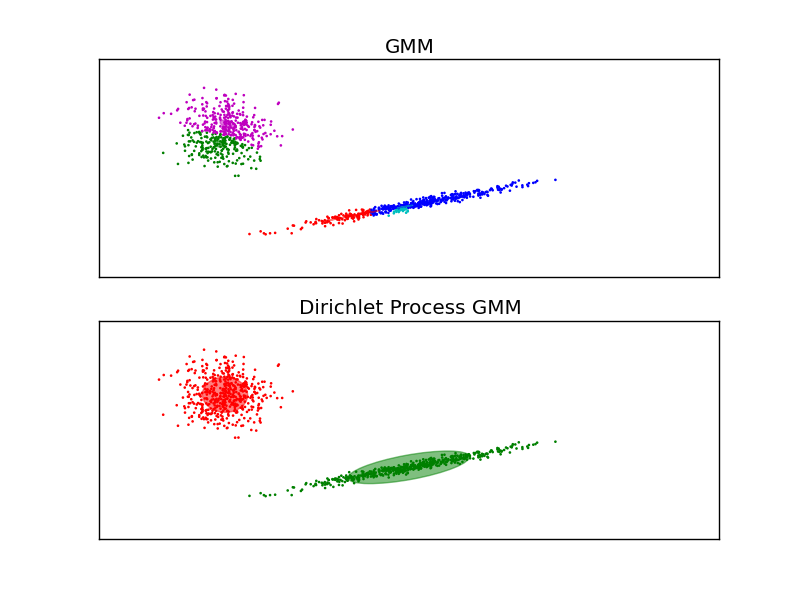
\includegraphics[scale=0.3]{images/plot_gmm_0011.png}
    \caption{\url{http://scikit-learn.org/stable/_images/plot_gmm_0011.png}}
    \end{figure}
\end{itemize}
\end{frame}


\begin{frame}
\frametitle{Dirichlet process mixture model}
\begin{itemize}
  \item What if you have a \emph{model} of the data? E.g. you know the 
    data is from a mixture of gaussian distributions. \pause

  \item What if there is no \emph{metric} on the data type? E.g. the data is
    categorical?
\end{itemize}
\end{frame}


\begin{frame}
\frametitle{Dirichlet process mixture model}
\begin{itemize}[<+->]
  \item The DPMM deals with these issues in a elegant framework.
  \item Describes the generative process
    of $n$ i.i.d. observations $Y_1, ..., Y_n$ as:
    \begin{align*}
      G &\sim \text{DirichletProcess}(\alpha, H) \\
      \theta_i | G &\sim G \\
      Y_i | \theta_i &\sim F(\theta_i)
    \end{align*} \pause
    where $F(\cdot)$ is a likelihood model (e.g. Gaussian),  $H(\cdot)$ is the
    \emph{prior} distribution (e.g. Normal-Inverse-Wishart) over the parameters
    of $F(\cdot)$, and $\alpha \in \R^{+}$ is chosen a-priori.
\end{itemize}
\end{frame}


\begin{frame}
\frametitle{Dirichlet process mixture model}
\begin{itemize}[<+->]
  \item The previous mathematical description is too abstract!
    \pause 
    (For instance, I didn't define what a 
    Dirichlet Process is...) 
    \pause
\end{itemize}
\end{frame}


\begin{frame}
\frametitle{Dirichlet process}
\pause
\begin{mydef}
Let $H(\cdot)$ be a measure over $\Set$ and $\alpha > 0$. We say $G$ is drawn
from a Dirichlet Process, written as $G \sim \text{DP}(\alpha, H)$ if for any
(measurable) partition of $\Set = (P_1, ..., P_n)$ we have
\begin{align*}
  (G(P_1), ..., G(P_n)) \sim \text{Dirichlet}(\alpha H(P_1), ..., \alpha H(P_n))
\end{align*}
\end{mydef}
\end{frame}


\begin{frame}
\frametitle{Wait... what?!}
\pause
Don't worry!  Alternative view known as the \textbf{Chinese Restaurant Process}
which is \emph{way} more intuitive.
\end{frame}


\begin{frame}
\frametitle{Chinese restaurant process}
\begin{itemize}[<+->]
  \item To make things more concrete and simple, let's say each $Y_i \in \{0,1\}^{D}$.
  \item Imagine a Chinese restaurant in SF with \emph{infinite} tables.
  \item Each table $T_i$ has a vector $\Theta^{(i)} = (\theta^{(i)}_1, ..., \theta^{(i)}_D)$, with
    each $\theta^{(i)}_j \sim \text{Beta}(\gamma, \beta),\; j{=}1,...,D$.
  \item To draw a value $Y_i$, first pick a table $T_j$, and then draw $Y_i \sim (\text{Bernoulli}(\theta^{(j)}_1), ..., \text{Bernoulli}(\theta^{(j)}_D))$.
  \item To reference our previous notation, $H=\text{Beta}(\gamma,\beta)^{D}$ and $F=\text{Bernoulli}(\cdot)^{D}$.
\end{itemize}
\end{frame}

\begin{frame}
\frametitle{Chinese restaurant process}
\begin{itemize}[<+->]
  \item So how do we pick a table?
  \item Suppose there are $n_j$ existing people at table $T_j$, and suppose we are the $n+1$-th observation.
  \item Pick table $T_j$ with probability $\frac{n_j}{n + \alpha}$, otherwise pick an empty table with probability $\frac{\alpha}{n + \alpha}$.
  \item Note: can prove that expected number of tables filled is $O(\alpha \log{n})$.
\end{itemize}
\end{frame}

\subsection{Inference}

\begin{frame}
\frametitle{How do we learn the model?}
\pause
Two major approaches:
\pause
\begin{itemize}[<+->]
  \item Markov chain Monte Carlo (e.g. Gibbs sampling)
  \item Variational methods 
\end{itemize}
\pause
\texttt{data-microscopes} only implements MCMC (for now!). 
\end{frame}

\begin{frame}
\frametitle{Gibbs sampling for DPMM}
\pause
\begin{block}{Problem statement}
Given $n$ data points $\Y = (Y_1, ..., Y_n)$, our goal is to learn the
distribution $p(\C | \Y)$, where $\C$ is the clustering (assignment vector) of $\Y$.
\end{block}
\pause
\textbf{Note:} when we say ``learn the distribution'' we mean draw
(independent) samples from.
\end{frame}


\begin{frame}
\frametitle{Gibbs sampling for DPMM}
Due to time constraints, please take on faith the following assertions:
\pause
\begin{itemize}[<+->]
  \item An exact analytical solution for $p(\C | \Y)$ is not readily available.
  \item Sampling $c_i^{(t)} \gets p(c_i | \C^{(t-1)}_{\neg i}, \Y), \;
    i=1,...,n$ over and over (and over) will \emph{eventually} get us $p(\C | \Y)$.
  \item The above strategy is called \emph{Gibbs sampling}.
\end{itemize}
\end{frame}


\begin{frame}
\frametitle{Gibbs sampling for DPMM}
To Gibbs sample, all we need to do is derive $p(c_i{=}k | \C_{\neg i}, \Y)$. 
\pause
\begin{align*}
  p(c_i{=}k | \C_{\neg i}, \Y) &\propto p(c_i{=}k, \C_{\neg i}, \Y) \\
                               &= p(c_i{=}k | \C_{\neg i}) p(Y_i | \Y^{(k)}) \\
                               &= p(c_i{=}k | \C_{\neg i}) \int_{\theta} p(Y_i | \theta) p(\theta | \Y^{(k)}) \; d\theta
\end{align*}
\pause

The $p(c_i{=}k|\C_{\neg i})$ term is easy to calculate given the CRP interpretation! \newline
\pause

If we pick $H$ and $F$ nicely, the integral on the RHS has an analytical solution!
\end{frame}


\begin{frame}
\frametitle{Gibbs sampling for DPMM}
Binary $Y_i \in \{0,1\}^{D}$ case, where $H$ is the Beta distribution and $F$
is Bernoulli, the Gibbs sampler distribution $p(c_i{=}k | \C_{\neg i}, \Y)$ is
(proportional to): \pause
\begin{align*}
  \frac{ |\Y^{(k)}_{\neg i}| }{ n - 1 + \alpha } \prod_{d=1}^{D} \frac{\left(\beta+\sum_{y_k\in \Y^{(k)}_{\neg i}} y_k^{(d)}\right)^{y_i^{(d)}} \left(  \gamma + |\Y^{(k)}_{\neg i}| - \sum_{y_k\in \Y^{(k)}_{\neg i}} y_k^{(d)}\right)^{(1-y_i^{(d)})} }{ \beta + \gamma + |\Y^{(k)}_{\neg i}| }
\end{align*}
when $k$ is an existing cluster and 
\pause
\begin{align*}
  \frac{ \alpha }{ n - 1 + \alpha } \prod_{d=1}^{D} \left(\frac{\beta}{\beta+\gamma}\right)^{y_i^{(d)}} \left(\frac{\gamma}{\beta+\gamma}\right)^{1-y_i^{(d)}}
\end{align*}
when $k$ is a new cluster.
\end{frame}


\section{Using data-microscopes}

\begin{frame}
\frametitle{Using \texttt{data-microscopes}}
\pause
\texttt{data-microscopes} implements what we talked about (and more!) 
\newline
\newline
\pause

\textbf{Now let's see the library in action!}
\end{frame}

%\begin{frame}[allowframebreaks]{References}
%\small
%\bibliographystyle{alpha}
%\bibliography{p}
%\end{frame}

\end{document}
